%%%%%%%%%%%%%%%%%%%%%%%%%%%%%%%%%%%%%%%%%
% Beamer Presentation
% LaTeX Template
% Version 1.0 (10/11/12)
%
% This template has been downloaded from:
% http://www.LaTeXTemplates.com
%
% License:
% CC BY-NC-SA 3.0 (http://creativecommons.org/licenses/by-nc-sa/3.0/)
%
%%%%%%%%%%%%%%%%%%%%%%%%%%%%%%%%%%%%%%%%%

%----------------------------------------------------------------------------------------
%	PACKAGES AND THEMES
%----------------------------------------------------------------------------------------

\documentclass{beamer}

    \mode<presentation> {
    
    % The Beamer class comes with a number of default slide themes
    % which change the colors and layouts of slides. Below this is a list
    % of all the themes, uncomment each in turn to see what they look like.
    
    %\usetheme{default}
    %\usetheme{AnnArbor}
    %\usetheme{Antibes}
    %\usetheme{Bergen}
    %\usetheme{Berkeley}
    %\usetheme{Berlin}
    %\usetheme{Boadilla}
    %\usetheme{CambridgeUS}
    %\usetheme{Copenhagen}
    %\usetheme{Darmstadt}
    %\usetheme{Dresden}
    %\usetheme{Frankfurt}
    %\usetheme{Goettingen}
    %\usetheme{Hannover}
    %\usetheme{Ilmenau}
    %\usetheme{JuanLesPins}
    %\usetheme{Luebeck}
    \usetheme{Madrid}
    %\usetheme{Malmoe}
    %\usetheme{Marburg}
    %\usetheme{Montpellier}
    %\usetheme{PaloAlto}
    %\usetheme{Pittsburgh}
    %\usetheme{Rochester}
    %\usetheme{Singapore}
    %\usetheme{Szeged}
    %\usetheme{Warsaw}
    
    % As well as themes, the Beamer class has a number of color themes
    % for any slide theme. Uncomment each of these in turn to see how it
    % changes the colors of your current slide theme.
    
    %\usecolortheme{albatross}
    %\usecolortheme{beaver}
    %\usecolortheme{beetle}
    %\usecolortheme{crane}
    %\usecolortheme{dolphin}
    %\usecolortheme{dove}
    %\usecolortheme{fly}
    %\usecolortheme{lily}
    %\usecolortheme{orchid}
    %\usecolortheme{rose}
    %\usecolortheme{seagull}
    %\usecolortheme{seahorse}
    %\usecolortheme{whale}
    %\usecolortheme{wolverine}
    
    %\setbeamertemplate{footline} % To remove the footer line in all slides uncomment this line
    %\setbeamertemplate{footline}[page number] % To replace the footer line in all slides with a simple slide count uncomment this line
    
    %\setbeamertemplate{navigation symbols}{} % To remove the navigation symbols from the bottom of all slides uncomment this line
    }
    
    \usepackage{graphicx} % Allows including images
    \usepackage{booktabs} % Allows the use of \toprule, \midrule and \bottomrule in tables
    %----------------------------------------------------------------------------------------
    %	TITLE PAGE
    %----------------------------------------------------------------------------------------
    
    \title[Question Classification]{Learning Question Classifiers} % The short title appears at the bottom of every slide, the full title is only on the title page
    
    \author{Yuchen Zhong} % Your name
    \institute[Tongji University] % Your institution as it will appear on the bottom of every slide, may be shorthand to save space
    {
        Tongji University \\ % Your institution for the title page
    \medskip
    \textit{} % Your email address
    }
    \date{\today} % Date, can be changed to a custom date
    
    \begin{document}
    
    \begin{frame}
    \titlepage % Print the title page as the first slide
    \end{frame}
    
    \begin{frame}
    \frametitle{Overview} % Table of contents slide, comment this block out to remove it
    \tableofcontents % Throughout your presentation, if you choose to use \section{} and \subsection{} commands, these will automatically be printed on this slide as an overview of your presentation
    \end{frame}
    
    %----------------------------------------------------------------------------------------
    %	PRESENTATION SLIDES
    %----------------------------------------------------------------------------------------
    
    %------------------------------------------------
    \section{Introduction} % Sections can be created in order to organize your presentation into discrete blocks, all sections and subsections are automatically printed in the table of contents as an overview of the talk
    %------------------------------------------------
    
    \begin{frame}
        \frametitle{Introduction}
        \begin{block}{}
        This paper introduces a two-layered classifiers to classifies
        questions. They used SNoW
        (which is a machine learnig system) to train and predict.
        \end{block}
        
        
        \textbf{Paper Highlights}
        \begin{itemize}
            \item hierarchical classifier
            \begin{itemize}
                \item \textbf{coarse classes}
                \item \textbf{fine classes}
            \end{itemize}
            \item machine learning approach
        \end{itemize}
    \end{frame}
    %------------------------------------------------

    \section{Question Classification} % A subsection can be created just before a set of slides with a common theme to further break down your presentation into chunks
    
    \subsection{Question Hierarchy}
    \begin{frame}
    \frametitle{Question Hierarchy}
    \begin{columns}[c]
        \column{.45\textwidth}
        a two-layered taxonomy
        \begin{itemize}
            \item 6 coarse classes
            \item 50 fine classes
        \end{itemize}

        \column{.5\textwidth}
        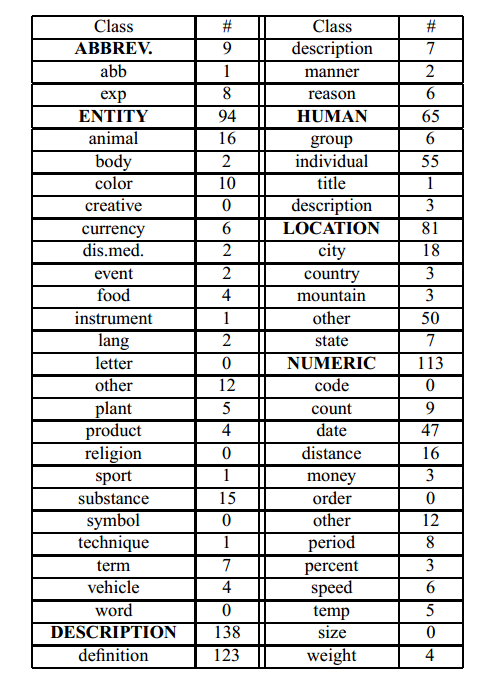
\includegraphics[scale=0.69]{1.png}

    \end{columns}
    
    \end{frame}
    
    \subsection{The Ambiguity Problem}
    \begin{frame}
    \frametitle{The Ambiguity Problem}
        \begin{block}{One Problem}
        There is no completely clear 
        boundary between classes.    
        \end{block}

        \begin{block}{Example}
            \begin{itemize}
                \item What is bipolar disorder?  
                \textbf{definition} or \textbf{disease\_medicine} 
                \item What do bats eat? 
                \textbf{animal} or \textbf{food}
                \item Waht is the PH scale? 
                \textbf{numeric value} or \textbf{definition}
            \end{itemize}                
        \end{block}

        \begin{block}{Solution}
            allow multiple class labels for a 
            single question. So it becomes a multi-labels
            problem.
        \end{block}
    \end{frame}

    %------------------------------------------------
    
    \section{Learning a Question Classifiers}

    \subsection{Process}
    \begin{frame}
        \frametitle{Process}
        \begin{columns}[c]
            \column{.48\textwidth}
            \begin{enumerate}
                \item $C_0$:The initial set of all the coarse classes
                \item $C_1$:The selected coarse classes by Coarse Classifier
                $|C_1| \leq 5$
                \item $C_2$:The corresponding fine classes determined by the class hierarchy
                \item $C_3$:The selected fine classes by Fine Classifier
                $|C_3| \leq 5$
            \end{enumerate}
            \column{.99\textwidth}
            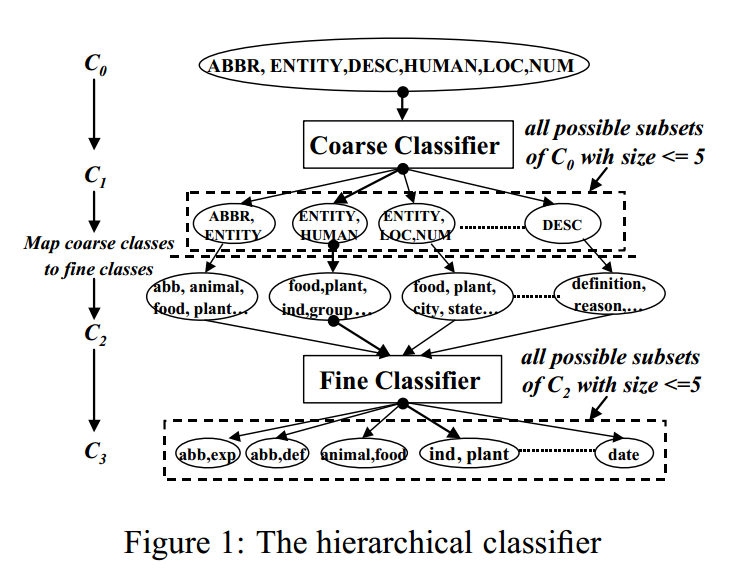
\includegraphics[scale=0.55]{2.png}
    
        \end{columns}
    \end{frame}

    \subsection{Features}
    \begin{frame}
        \frametitle{Features}
        \begin{block}{}
            Each question is analyzed and 
            represented as a list of features
        \end{block}
        \begin{block}{Primitive Features}
            \begin{itemize}
                \item words
                \item pos tags 
                \item chunks 
                \item named entities
                \item head chunks 
                \item semantically related words(RelWord)
            \end{itemize}
        \end{block}
        \begin{block}{Complex features}
            \begin{itemize}
                \item conjunctive(n-grams)
                \item relational features
            \end{itemize}
        \end{block}
    \end{frame}


    \subsection{Decision Model}
    \begin{frame}
        \begin{block}{Model——SNoW}
            SNoW is a machine learning system 
            developed in 1998. Its main algorithm
            is Winnow algorithm. SNoW deals with 
            multi-class problems and will return 
            possibilities of each class.
        \end{block}

        \begin{block}{Details}
            Given a confusion set and a question,
            SNoW outputs possibilities of each class
            ($P=\{p_1,p_2,...,p_n\}$).
            Select the highest k classes($k \leq 5$) where
            k satisfies, 
            \[
                k = \min(\arg\min_t(\sum_{i=1}^{t}p_i \geq T),5)
            \]
            T is a threshold and $T=0.95$ in the experiments.
        \end{block}


    \frametitle{Decision Model}
        
    \end{frame}
    %------------------------------------------------

    \section{Results}

    \begin{frame}
    \frametitle{Results}
         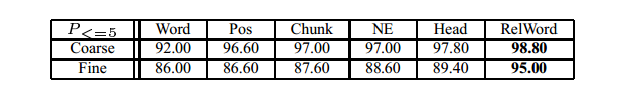
\includegraphics{3.png}   
         
         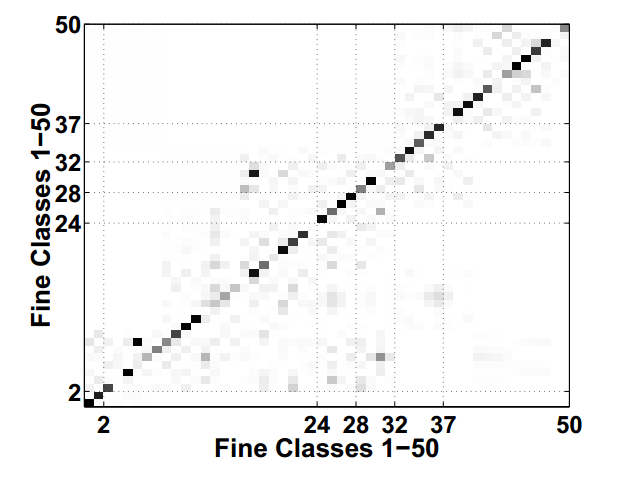
\includegraphics[scale=0.75]{4.png}
    \end{frame}


    %------------------------------------------------
    \begin{frame}
    \Huge{\centerline{The End}}
    \end{frame}
    
    %----------------------------------------------------------------------------------------
    
    \end{document}